\subsection{MEX 2-1a: Pressure driven percolation, Saltstone}

Participating institutions of MEX 2-1a (see section \ref{sec:mex02}): CAU, UFZ, IfG

\subsubsection*{UFZ}

Link to the data set at UFZ data investigation portal (Download only for project members):
\url{https://www.ufz.de/record/dmp/archive/7706/}

The link contains two input decks for OGS-6 in which pressure driven percolation as described in MEX2 is simulated under different configurations of boundary loading.
The first case applies the boundary loading of 12 MPa, 21 MPa, and 8 MPa in x-, y-, and z-direction respectively. It is called ''case 1" and the corresponding OGS-6 input file is ''me2\_insitu\_case1.prj".
The second case is loaded with 4 MPa, 15 MPa, and 19 MPa in x-, y-, and z-direction respectively and the input file is named ''me2\_insitu\_case2.prj".
The remaining files are vtu files that describe the computing domain and the boundaries as shown in~\ref{fig:VPF_init}.

\begin{table}[!ht]
\caption{MEX 2-1a (UFZ): Meta Data according to Dublin Core}
\label{tab:dms-mex2-1a-ufz}
\small
\begin{tabular}{R{3.5cm}|L{7.5cm}}
\hline
%
Data label & MEX 0-1a (UFZ) \\
URL & \url{https://www.ufz.de/record/dmp/archive/7706/} \\ 
Subject  & Bending fracture test \\
Type of data  & Data set (structured data in a defined format) \\
Data quality  & Quality assured data by benchmarking \\
Status of data  & Processed data \\
Data format  & OGS files \\
Creators  & Yoshioka, Keita  \\
Source/Origin & Open source \\
Publisher  & Helmholtz Centre for Environmental Research UFZ \\
Rights holders & Helmholtz Centre for Environmental Research UFZ \\
Contributors & Yoshioka, Keita; Wang Wenqing \\
Time/period of creation & 2019-2020 \\
Language of content & English \\
Update policy & To be merged to OGS benchmarks (see below) \\
Access permissions & Free access \\
%
\hline
\end{tabular}
\end{table}

MEX 2-1a (UFZ) will be also provided as an OGS benchmark case at:\\
\small
\url{https://www.opengeosys.org/docs/benchmarks/phase-field/phasefield/}
\normalsize

\subsubsection*{CAU Kiel}

The required LEM code and the input variables of the percolation test on saltstone samples are uploaded to the IfG (Kiel) NextCloud server. The data is accessible through the following link:\\
\hyperlink{https://nextcloud.ifg.uni-kiel.de/index.php/s/9JZZcpS4S3JJT9S}{https://nextcloud.ifg.uni-kiel.de/index.php/s/9JZZcpS4S3JJT9S}\\

The uploaded protected MATLAB file in a *.p format requires a MATLAB version with a built-in Voronoi Tessellation and Delaunay Triangulation functions. The input variables are prepared in two files for two different stress configurations. Fig. \ref{fig:Amir_ME2_LEM_b_model_Fracture_Data} shows the frack surfaces under the percolation test as described in section \ref {sec:mex02}.

\begin{figure}[!ht]
\centering
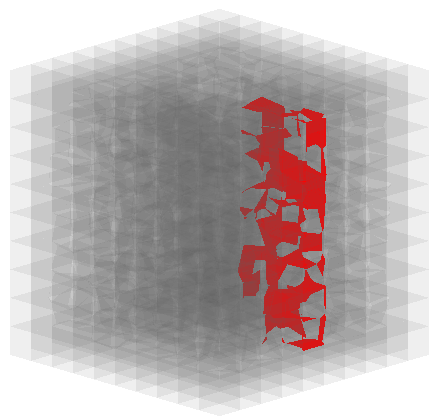
\includegraphics[width=4cm,height=4cm]{figures/Amir_ME2_LEM_b_model_Fracture_Data.png}
\caption{The frack surfaces (red) under the percolation test, Saltstone}
\label{fig:Amir_ME2_LEM_b_model_Fracture_Data}
\end{figure}

\begin{table}[!ht]
\caption{MEX 2-1a: Pressure driven percolation, Saltstone}
\label{tab:dms-mex2-1a-cau}
\small
\begin{tabular}{R{3cm}|L{7cm}}
\hline
%
Data label & GeomInt | CAU | Percolation test, Saltstone\\
URI &  https://nextcloud.ifg.uni-kiel.de/index.php/s/9JZZcpS4S3JJT9S (Numerics)
\\
Subject  &  Percolation test, Saltstone\\
Type of data  & executable MATLAB P-file, input parameters\\
Dataquality  &  quality assured data \\
Status of data  &  unprocessed data\\
Dataformat  & txt, MATLAB executable P-file\\
Creators  &  Kiel University, Institute of Geomechanics and Geotechnics, Ludewig-Meyn-Stra\ss e 10, 24118, Kiel\\
Source/Origin & In-house code \\
Publisher  &  Kiel University, Institute of Geomechanics and Geotechnics, Ludewig-Meyn-Stra\ss e 10, 24118, Kiel \\
Rights holders &  Kiel University, Institute of Geomechanics and Geotechnics, Ludewig-Meyn-Stra\ss e 10, 24118, Kiel \\
Contributors &   Kiel University, Institute of Geomechanics and Geotechnics: Amir Shoarian Sattari, Frank Wuttke\\
Time or Period of creation &  2018-2020\\
Language of the content &  English\\
Update policy &  stored data is final\\
Access permissions & full access\\
%
\hline
\end{tabular}
\end{table}